\documentclass[../tesis_main.text]{subfiles}

%%%%%%%%%%%%%%%%%%%%%%%%%%%%%%%%%%%%%%%
%   Agregar refencias al papper de Justina
%	Describir constitución del robot
%

\chapter{Marco teórico}
	\section{Robots de servicio}
		%Conceptos


		%Estado del arte
		Dado que este trabajo se centrará en los robots de servicio es importante mencionar que un robots de servicio es un robot capaz de realizar tareas de la vida diaria en un ambiente similar al de un hogar real. Actualmente el desarrollo de este tipo de robot está guiado por la competencia internacional Robocup @Home.\cite{robocupAtHome} Esta categoría promueve la incorporación de habilidades robóticas avanzadas para la interacción con los humanos y con el entorno de operación. Esta competencia se enfoca a desarrollar habilidades en los robots de servicios. Ejemplos de estas habilidades son la localización y navegación segura en ambientes no controlados, la comunicación natural humano-robot por voz y gestos y habilidades visuales para el reconocimiento y la manipulación de objetos.\cite{femexrobotics}\\

		Los robots de servicio enfrentan diversos retos: desarrollar tareas en ambientes dinámicos, características de entornos no estandarizados, incertidumbre ante escenarios desconocidos. Dadas las condiciones en que estos robots operan los programadores y desarrolladores de robots de servicios han optado por dotar a los robots de ciertas capacidades. Por ejemplo el robot Cosero, consta de un sistema de percepción del entorno, un sistema de manipulación, un sistema de interacción humano-robot y un sistema de planeación de tareas.\\ %%%%REFFFFFF

		\textit{Tabla con las características de los robots de servicio.}\\

		\begin{figure}[htb]
			\begin{center}
			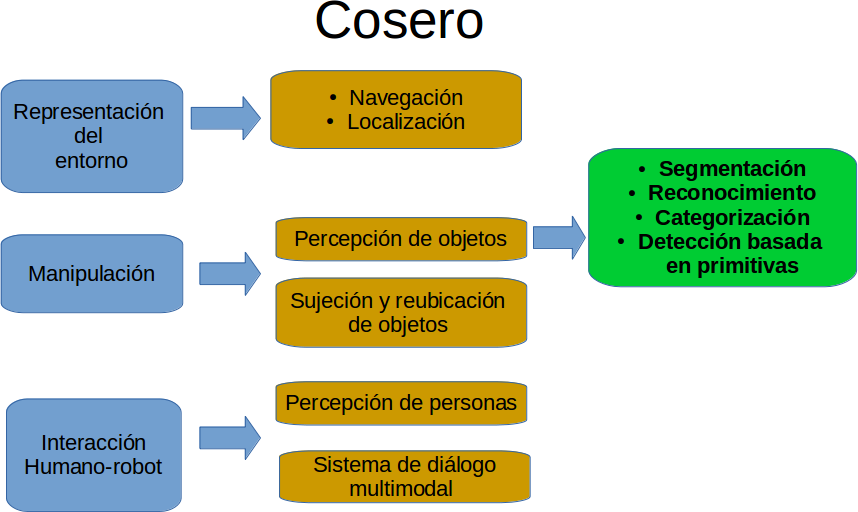
\includegraphics[width=8.5cm, height=5cm]{estadoArte/cosero.png}
			\caption{Estructura de software del robot Cosero.}
			\end{center}
		\end{figure}

		\begin{figure}[htb]
			\begin{center}
			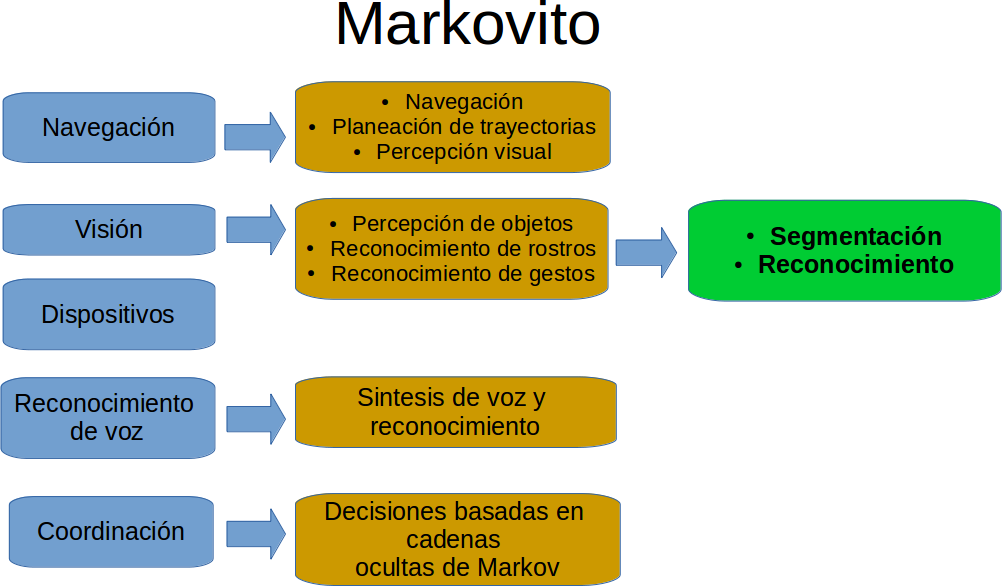
\includegraphics[width=8.5cm, height=5cm]{estadoArte/markovito.png}
			\caption{Estructura de software del robot Markovito.}
			\end{center}
		\end{figure}

		\begin{figure}[htb]
			\begin{center}
			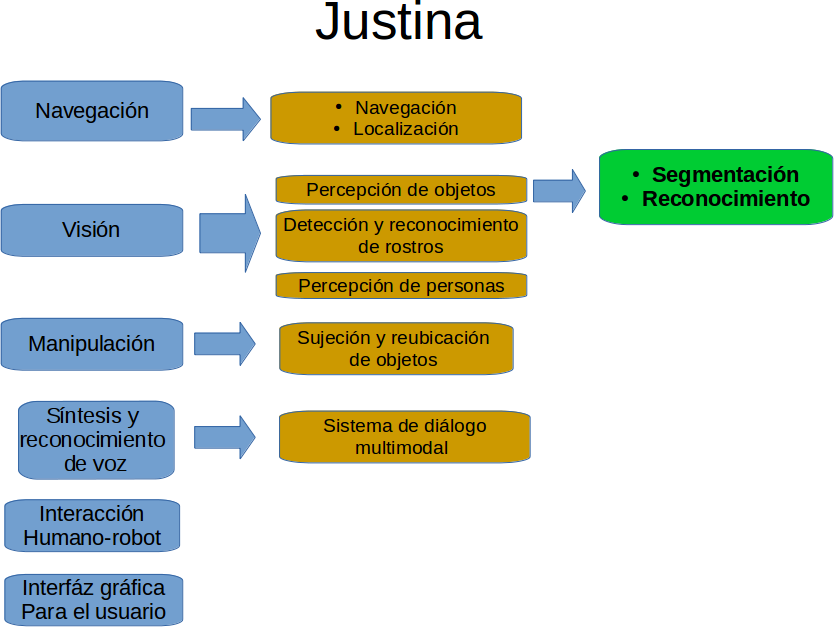
\includegraphics[width=8.5cm, height=5cm]{estadoArte/justina.png}
			\caption{Estructura de software del robot Justina.}
			\end{center}
		\end{figure}

		En particular en una metodología de detección y manipulación de objetos, resulta una tarea fundamental a resolver en los robots de servicio. La idea general de la robótica de servicio doméstico ha existido desde hace mucho tiempo, pero es un tema de investigación relativamente joven. El objetivo de crear robots de servicios útiles y autónomos que puedan interactuar con seres humanos y objetos en el mundo real en un entorno natural plantea un gran número de problemas sin resolver en muchas disciplinas científicas.\\
		%\vspace{0.2in}

		Recientemente, el progreso en estos campos de investigación, así como el progreso y la normalización en el desarrollo de hardware y software, ha llevado a un aumento en la disponibilidad de recursos, métodos y componentes para el desarrollo  de Robots de servicio doméstico . Por ello estamos cada vez más cerca de convivir con robots de servicios de manera exitosa en diversos lugares, por ejemplo hospitales \cite{hospitalRobots}, oficinas, construcciones, o tiendas departamentales \cite{robotsInStores}.\\
		%\vspace{0.2in}


		Estos desarrollos han sido posibles gracias a herramientas de código abierto como lo es Ubuntu, ya que ha servido como base para el desarrollo de software especializado para robots, por ejemplo ROS \cite{rosEpage}. Este conjunto de librerías especializadas para robots pueden llegar a ser muy particulares y estar enfocados a una sola área de investigación de las antes mencionadas, por ejemplo: Carmen \cite{carnegieMellon}, un conjunto de librerías y algoritmos de control para navegación de robots, desarrollados por la universidad Carnegie Mellon\cite{cMellonEpage}.\\
		%\vspace{0.2in}

		En la parte de simulación se cuenta con ejemplos como el USARSim \cite{balakirsky2006}, rviz \cite{rVizEpage} o Gazebo \cite{gazeboEpage}. Por lo que respecta a los algoritmos de visión computacional existen bibliotecas de código abierto por ejemplo OpenCV \cite{openCV} el cual tiene un gran campo de aplicaciones\cite{bradski2000}. Por lo que corresponde a los kits estándar de hardware, podemos mencionar la construcción de robots de plataforma estándar por ejemplo VolksBot \cite{wisspeintner2007} y las plataformas bases por ejemplo ActivRobots \cite{ActivRobots}, Pepper \cite{pepperEpage}, Asimo \cite{asimoEpage} ha hecho posible desarrollar software de manera más rápida y eficiente.\\
		%\vspace{0.2in}

		\begin{figure}[htb]
			\begin{center}
			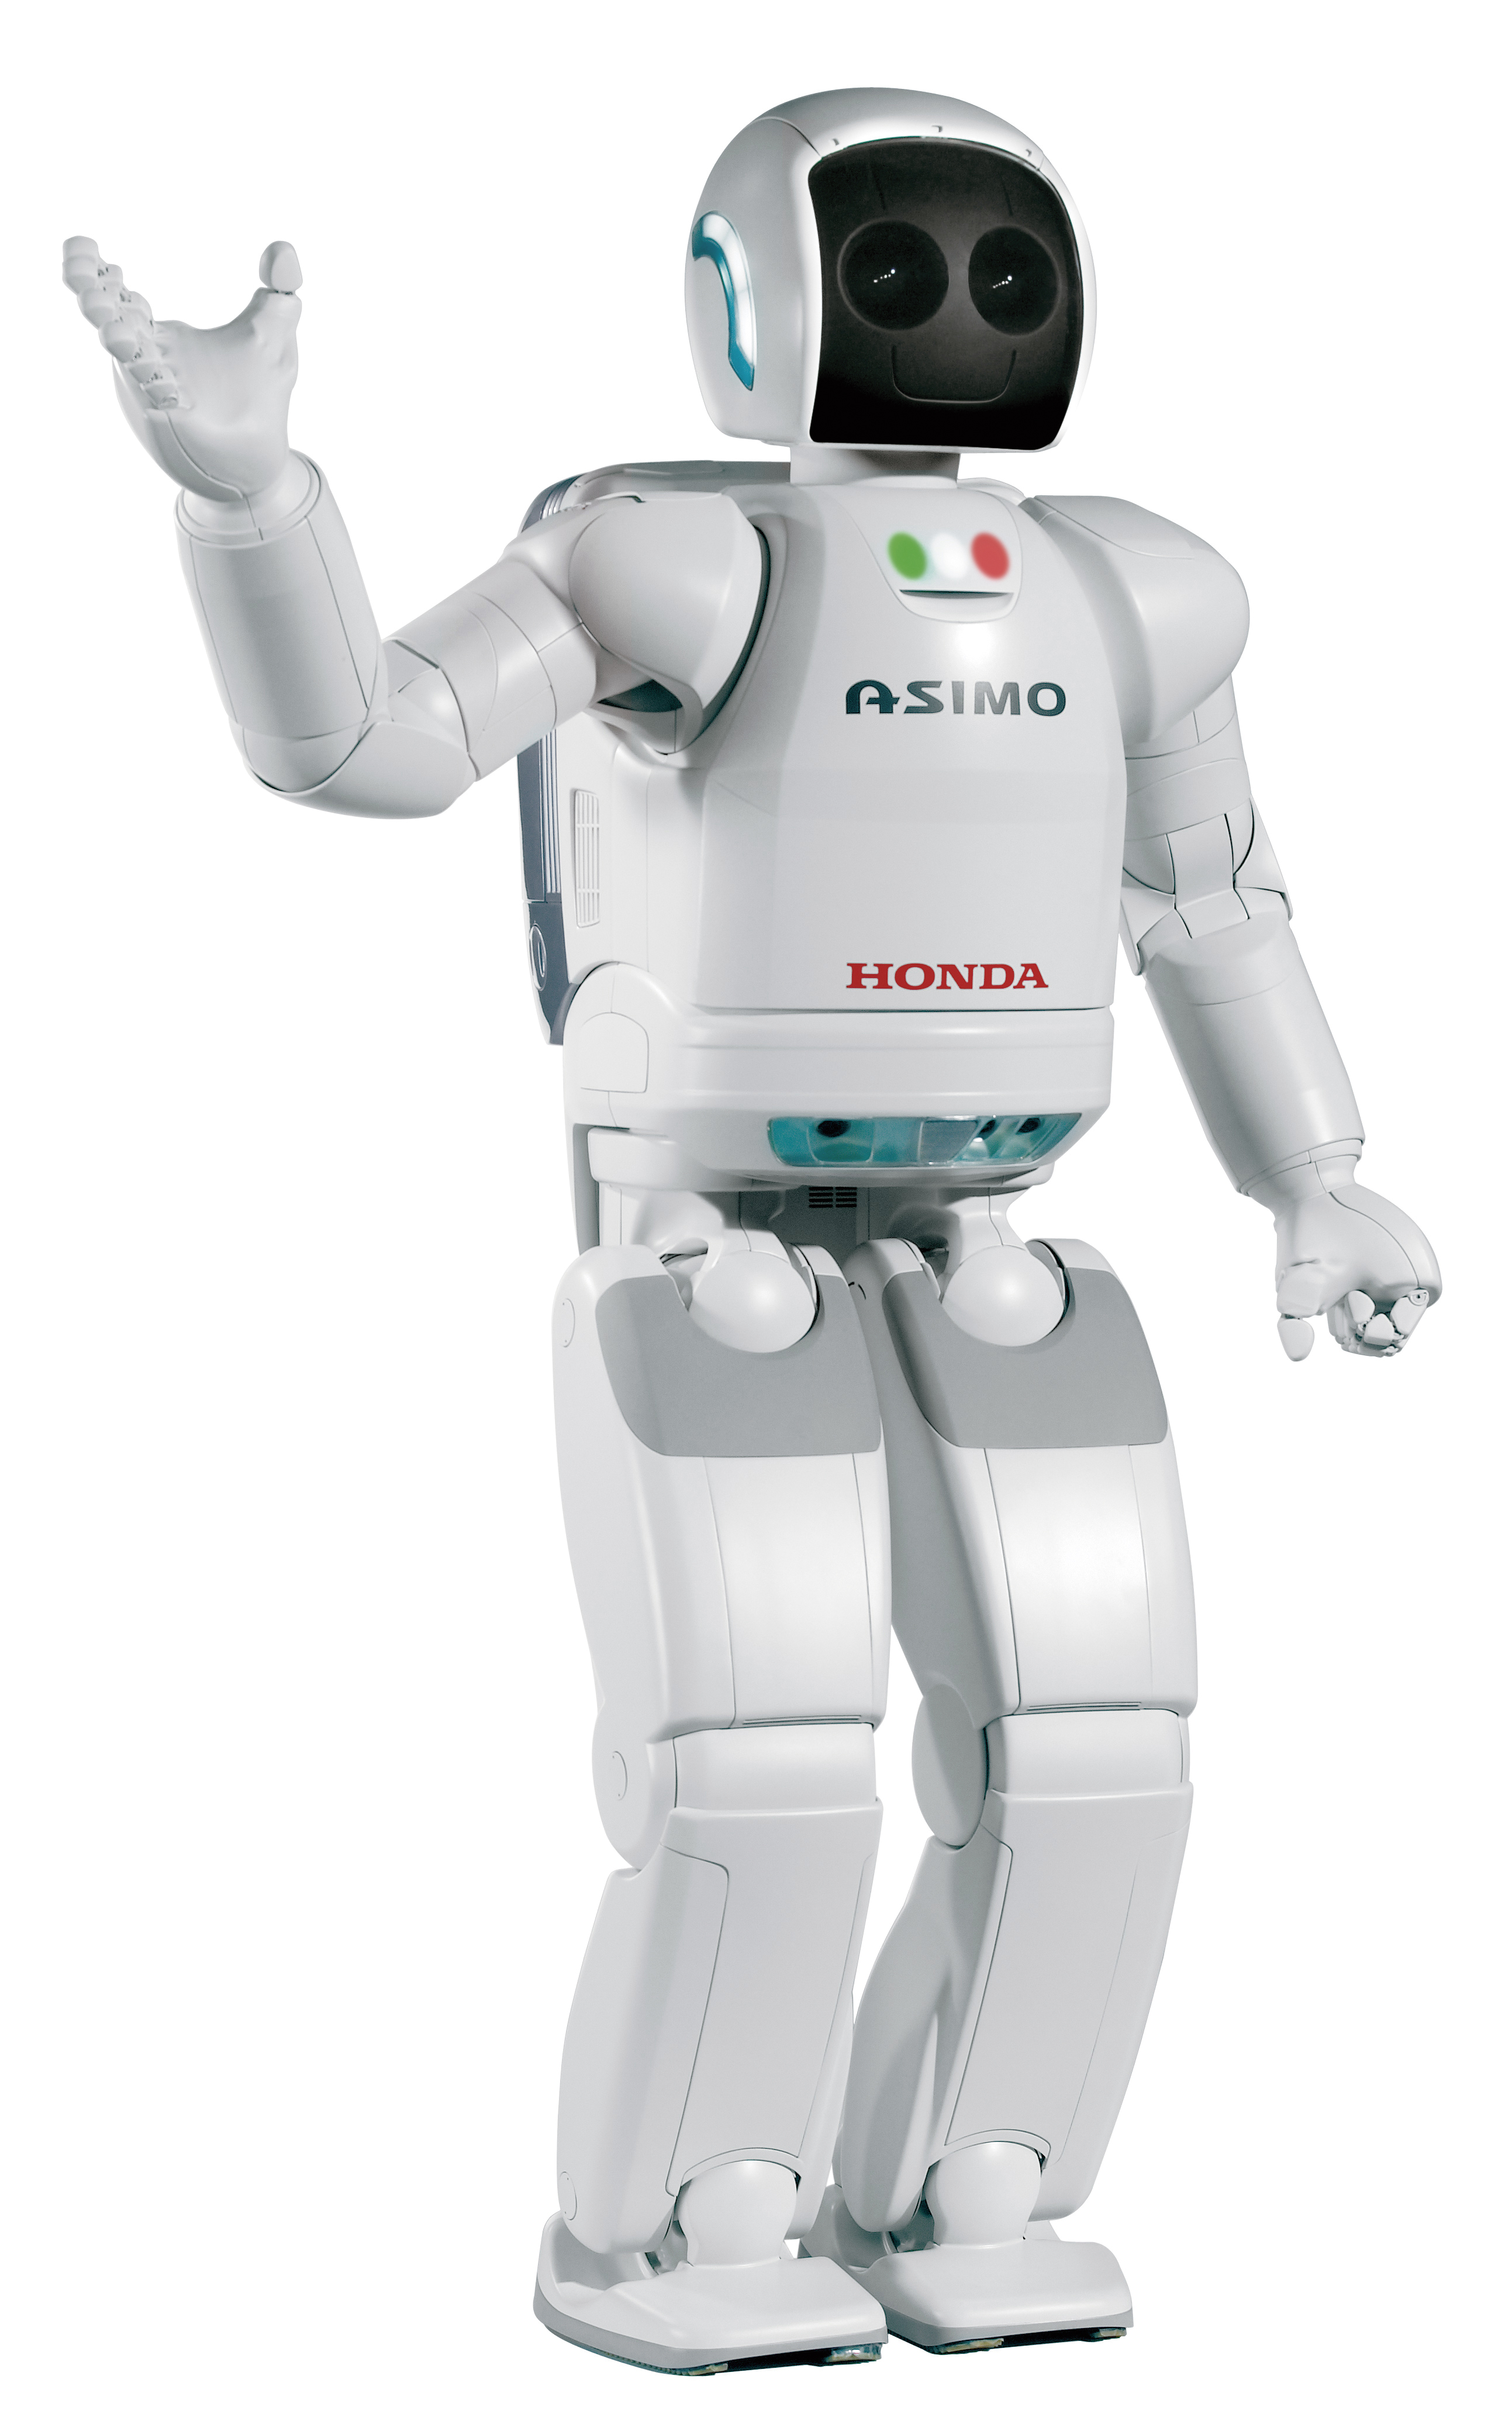
\includegraphics[width=3.5cm, height=5cm]{estadoArte/asimo.jpg}
			\caption{Robot asimo desarrollado por la compañía Honda.}
			\end{center}
		\end{figure}



%%% Fundamentos de Manipuladores
%%  ---------------------------------

	\section{Fundamentos básicos de Robots Manipuladores}
		La manipulación adecuada de objetos es una característica imprescindible en los robots de servicio dadas las condiciones de su entorno y las tareas cotidianas que le podemos asignar a dicho robot. Una posible solución a la problemática de la manipulación de objetos es la incorporación de manipuladores seriales a una base móvil; sin embargo se debe tener en cuenta que los objetos a ser manipulados se encuentran en condiciones aleatorias de posición y orientación, estas características implican que el manipulador serial debería ser capaz de alcanzar una posición (x, y, z) con cualquier orientación (roll, pitch, yaw).\\

		Los robots manipuladores clásicos presentan una configuración antropomórfica serial, que hace semejanza con un brazo humano. La arquitectura típica de un manipulador consiste en una serie de barras rígidas unidas entre sí mediante el uso de articulaciones rotacionales o prismáticas. De manera general cada articulación logra su movimiento gracias a un actuador y a la adición de algunos elelmentos complementarios como sensores de posición y de velocidad\cite{baturone2005}.\\

		Los robots manipuladores clásicos están caracterizados, desde el punto de vista mecánico, por una serie de propiedades tales como los grados de libertad, el espacio de trabajo, la rigidez estructural, peso propio y la capacidad de llegar a un punto deseado con exactitud en múltiples repeticiones. Además en los robots manipuladores suelen tomarse en cuenta otras características adicionales: la carga útil máxima y la velocidad de trabajo.\\

		\begin{figure}[htb]
			\begin{center}
			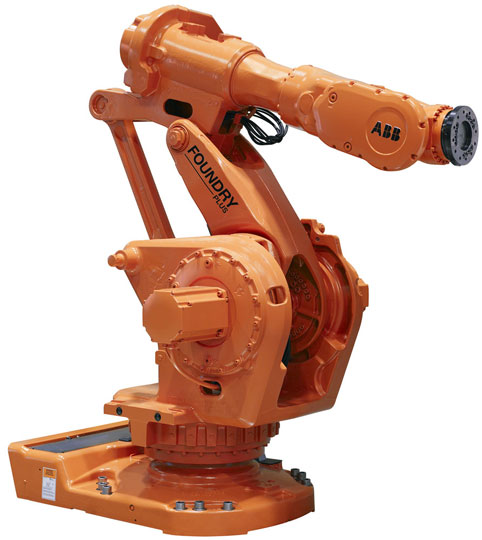
\includegraphics[width=3.5cm, height=4cm]{estadoArte/serial_abb.jpg}
			\caption{Robot serial elaborado por la compañía ABB.}
			\end{center}
		\end{figure}

		\subsection{Configuraciones típicas y parámetros característicos}
			Según la geometría de su estructura mecánica, un manipulador puede ser:

			\begin{itemize}
				\item{Cartesiano, cuyo posicionamiento en el espacio se lleva a cabo mediante articulaciones lineales.}

				\item{Cilíndrico, con una articulación rotacional sobre una base y articulaciones lineales para el movimiento en altura y en radio.}

				\item{Polar, que cuenta con dos articulaciones rotacionales y una lineal.}

				\item{Esférico (o de brazo articulado), con tres articulaciones rotacionales.}

				\item{Mixto, que posee varios tipos de articulaciones, combinaciones de las anteriores. Es destacable la configuración SCARA (Selective Compliance Assembly Robot Arm).}

				\item{Paralelo, posee brazos con articulaciones prismáticas o rotacionales concurrentes. Figura 2.3}
			\end{itemize}

Los principales parámetros que caracterizan a los robots industriales son:

	\begin{itemize}
		\item{Número de grados de libertad. Es el número total de grados de libertad de un robot, dado por la suma de g.d.l. de las articulaciones que lo componen. Aunque la mayoría de las aplicaciones industriales requieren 6 g.d.l., como las de soldadura, mecanizado y almacenamiento, otras más complejas requieren un número mayor, tal es el caso de las labores de montaje.}

		\item{Espacio de accesibilidad o espacio (volumen) de trabajo. Es el conjunto de puntos del espacio accesibles al punto terminal, que depende de la configuración geométrica del manipulador. Un punto del espacio se dice totalmente accesible si el efector final puede situarse en él en todas las orientaciones que permita la constitución del manipulador y se dice parcialmente accesible si es accesible por el efector final pero no en todas las orientaciones posibles. En la figura inferior se aprecia el volumen de trabajo de robots de distintas configuraciones.}

		\item{Capacidad de posicionamiento del punto terminal. Se concreta en tres magnitudes fundamentales: resolución espacial, precisión y repetibilidad, que miden el grado de exactitud en la realización de los movimientos de un manipulador al realizar una tarea programada.}

		\item{Capacidad de carga. Es el peso que puede transportar el elemento terminal del manipulador. Es una de las características que más se tienen en cuenta en la selección de un robot dependiendo de la tarea a la que se destine.}

		\item{Velocidad. Es la máxima velocidad que alcanzan el efector final y las articulaciones.}
	\end{itemize}

		\begin{figure}[htb]
			\begin{center}
			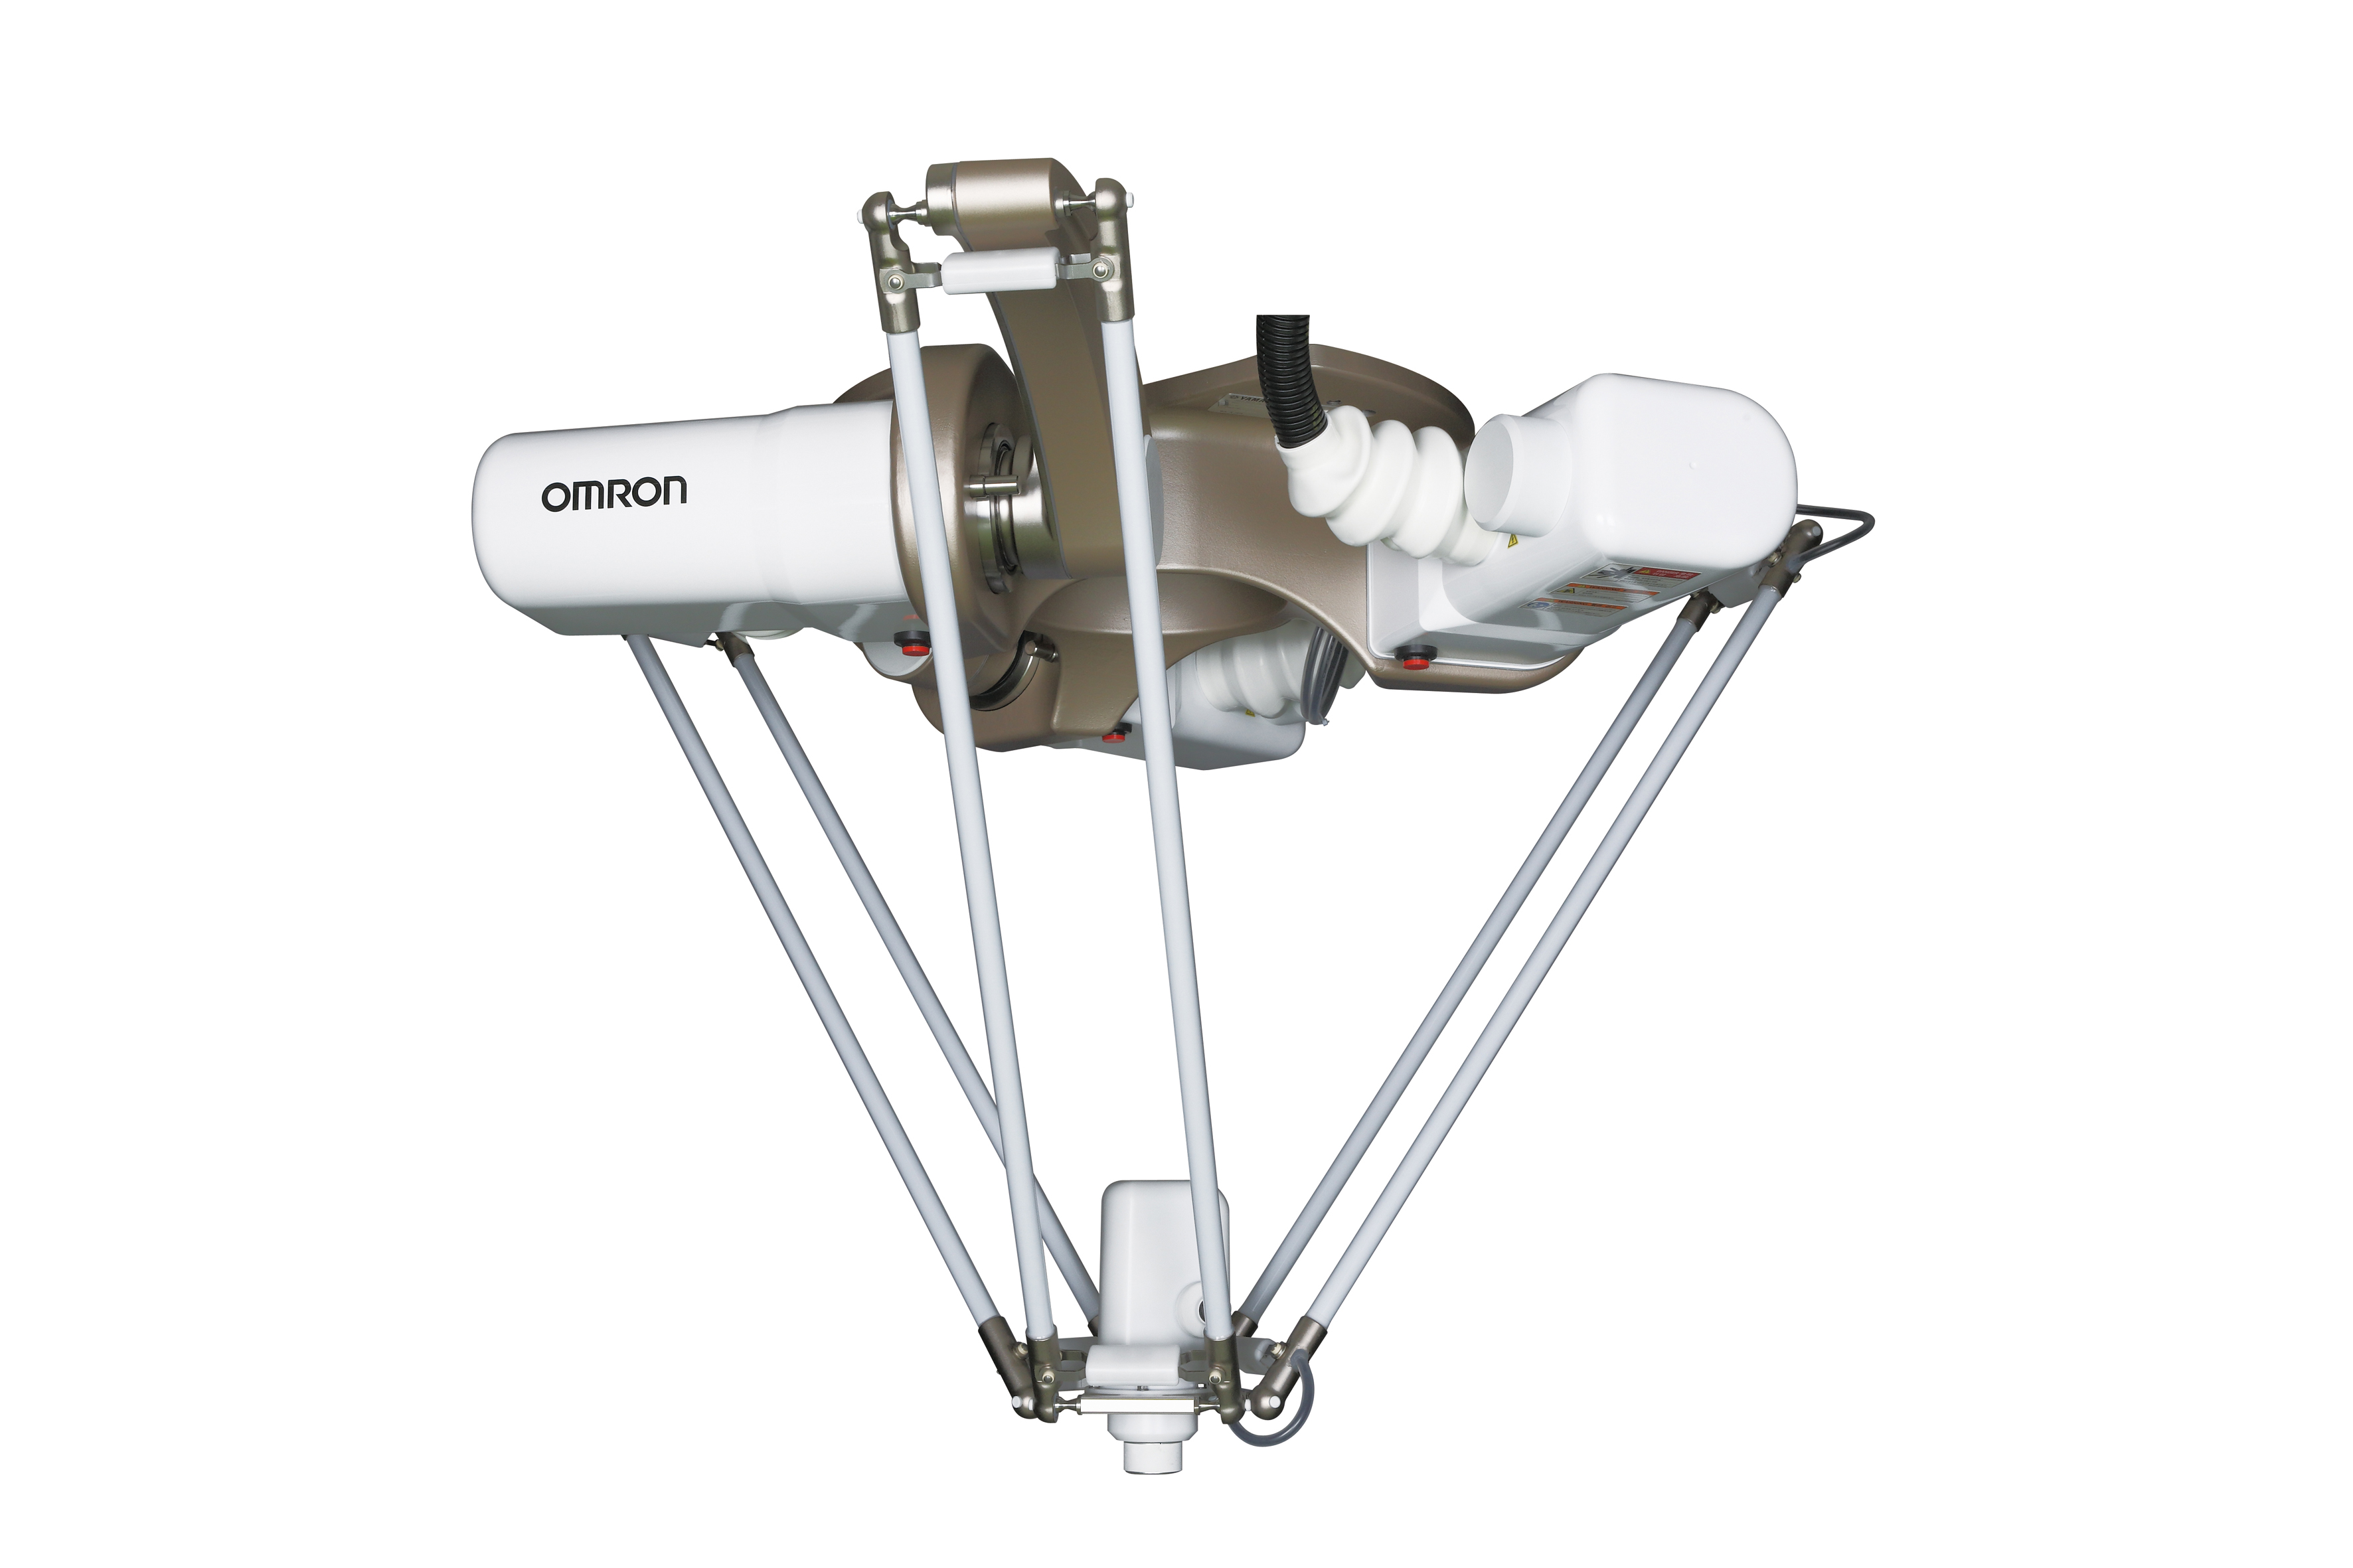
\includegraphics[width=6.5cm, height=4.5cm]{estadoArte/robotParalelo.jpg}
			\caption{Robot paralelo.}
			\end{center}
		\end{figure}


		\subsection{Descripciones espaciales y transformaciones}
			La cinemática es la ciencia del movimiento que trata el tema sin considerar las fuerzas que lo ocasionan. Dentro de esta ciencia se estudian la posición, la velocidad y la aceleración. En consecuencia, el estudio de la cinemática de manipuladores se refiere a todas las propiedades geométricas y las basadas en los cambios de estas a lo largo del tiempo. Dadas las características de este trabajo solo se abordarán la cinemática directa e inversa, sin llegar a analizar la dinámica del manipulador.\\

			El problema de la cinemática directa se plantea en términos de encontrar una matriz de trasformación que relaciona el sistema de coordenadas ligado al cuerpo en movimiento respecto a un sistema de coordenadas que permanece estático y se toma como referencia. Para lograr esta representación se usa la matriz de transformación homogénena con una dimensión 4x4, la cual incluye las operaciones de rotación y translación.\\

			La matriz de transformación homogénea es una matriz de 4x4 que transforma un vector expresado en coordenadas homogéneas desde un sistema de coordenadas hasta otro sistema de coordenadas. La matriz de transformación homogénea tiene la siguiente estructura:\\

			
			$$
			T_0 ^ 1  =
			\begin{bmatrix}
    			n_{x} & s_{x} & a_{x} &  p_{x} \\
			    n_{y} & s_{y} & a_{y} &  p_{y} \\
			    n_{z} & s_{z} & a_{z} &  p_{z} \\
			    0     &   0   &   0   &    1
			\end{bmatrix}
			$$

			donde los vectores n, s, a, son vectores ortogonales unitarios que representan la rotación del sistema y p es un vector que describe la posición x, y, z del origen del sistema actual respecto del sistema de referencia.

			\begin{SCfigure}
				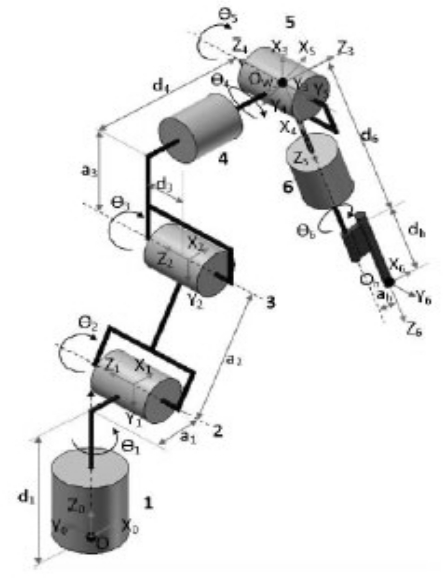
\includegraphics[width=4.5cm, height=6.5cm]{estadoArte/esquema_serial.jpg}
				\caption{Esquema de sistemas de referencia en robot antropomórfico de seis grados de libertad.}
			\end{SCfigure}


		\subsection{Cinemática directa}
			El problema de la cinemática directa consiste en determinar la posición del efector final en el espacio dado el valor de cada una de las articulaciones. El valor de los ángulos de las articulaciones se determinan con ayuda de sistemas de referencia ubicados en cada una de las articulaciones del robot.\\

			Un robot manipulador está compuesto de un conjunto de enlaces conectados por varias juntas. Las articulaciones pueden ser muy simples, tales como una articulación de revolución o una articulación prismática. Una articulación de revolución es como una bisagra y permite una rotación relativa alrededor de un solo eje coordenado; una junta prismática permite un movimiento lineal a lo largo de un solo eje. En ambos casos podemos observar el que la articulación tiene un solo grado de libertad de movimiento: el ángulo de rotación en el caso de una articulación de revolución, y la cantidad de desplazamiento lineal en el caso de una articulación prismática.\\

			Con el supuesto de que cada articulación tiene un solo grado de libertad, la acción de cada una de las articulaciones se puede describir por un solo número real: el ángulo de rotación en el caso de una articulación de revolución o el desplazamiento en el caso de una junta prismática. El objetivo del análisis de la cinemática directa es determinar el efecto acumulativo de todo el conjunto de variables de la articulación y observarlo en el efector final.\cite{spong2008robot}\\

			El análisis cinemático de un manipulador de n-enlaces puede ser extremadamente complejo y las convenciones que se presentan a continuación simplifican el análisis considerablemente.\\

			Un robot manipulador con $n$ grados de libertad tendrá por consecuencia n articulaciones. Se numeran las articulaciones de 1 a $n$, y se numeran los enlaces de $0$ a $n$, comenzando desde la base en un sistema de referencia fijo. Para esta convención, la articulación $i$ conecta el enlace $i - 1$ al enlace $i$.\\

			Cuando se acciona la articulación i el enlace se mueve, por lo tanto, el enlace 0 (el primer eslabón) es fijo, y no se mueve cuando las juntas consecuentes son accionadas. Por supuesto, el robot manipulador podría ser móvil (por ejemplo, podría ser montado en una plataforma móvil o en un vehículo autónomo), pero para esta primer parte abordaremos el problema suponiendo una plataforma fija.\\




%%  Imagenes RGD y Points Clouds
%%  ----------------------------------------------
	\section{Imágenes RGB-D}
		En la robótica de servicios resulta imprescindible contar con robots que sean capaces de percibir su entorno, los elementos que los rodean y determinar características de los mismos. Los humanos, dadas estas necesidades, hemos desarrollado el sentido de la vista que nos permite determinar características del entorno y de los objetos que lo componen tales como el color, la forma, las dimensiones ó su ubicación en el espacio.\\

		Para optimizar los movimientos de un robot, no sólo se debe identificar cada objeto que se encuentra en el entorno de trabajo, sino también la posición que estos guardan respecto al robot. Normalmente, la segmentación de objetos de una imagen se logra mediante la segmentación de color, esta segmentación se logra a partir del análisis cromático de los componentes RGB de la imagen obtenida del objeto; sin embargo, este método es poco eficiente debido a que es sumamente suceptible a los cambios en la iluminación. \cite{objectDetectingKinect}\\ 

		Por lo tanto, necesitamos considerar una fuente de datos adicional, en este caso la profundidad, para discriminar objetos que no están en el rango de interés. En este documento se reportan los datos obtenidos al resolver este problema con la incorporación de un sensor RGB-D.\\

		La rápida evolución de esta reciente tecnología ha resultado en el aumento de la calidad de las imágenes, la mejora en la sincronización del color con la profundidad y la disminución del tiempo de muestreo entre cada imagen. En particular, la profundidad de la imagen se obtiene en una matriz resultado de la proyección de rayos infrarrojos sobre los objetos. El sensor cuenta con una cámara infrarroja que obtiene la lectura de los haces infrarrojos reflejados sobre los objetos.\\

		El sensor Kinect incorpora un sensor de profundidad, un cámara de color y un arreglo de cuatro micrófonos que, en conjunto, proporcionan una captura de movimiento de cuerpo completo en 3D. La figura 2.5 muestra la disposición del proyector de infrarrojos (IR), la cámara de color y la cámara IR. El sensor de profundidad consta de un proyector IR combinado con una cámara IR, la cual es un sensor semiconductor de metal-óxido monocromático. El sensor de profundidad es desarrollado por la compañía israelí PrimeSense.\\

		Aunque la tecnología exacta es cerrada, se basa en el principio de la estructura de la luz y su difracción. El proyector IR es un láser IR que pasa a través de una rejilla de difracción y se esparce como una nube de puntos. Dada la geometría de construcción entre el proyector IR y la cámara IR se puede reconstruir un modelo 3D si se observa un punto en el proyector y posteriormente se ubica su correspondiente reflexión en la cámara, esto se puede lograr utilizando triangulación.\\

		Debido a que el patrón de puntos es relativamente al azar, la coincidencia entre la imagen IR y el patrón del proyector puede realizarse de forma directa comparando pequeñas vecindades utilizando, por ejemplo, referencias cruzadas.\cite{kinectFeatures}\\

		El valor de la profundidad se codifica en escala de grises, cuanto más oscuro sea un píxel, más cerca está el punto de la cámara en el espacio, los píxeles negros indican que no se posee información respecto a la distancia en ese píxel. Esto puede suceder si los píxeles están demasiado lejos o demasiado cerca de la cámara IR.\\

		\begin{figure}

			\begin{subfigure}[t]{.5\textwidth}
			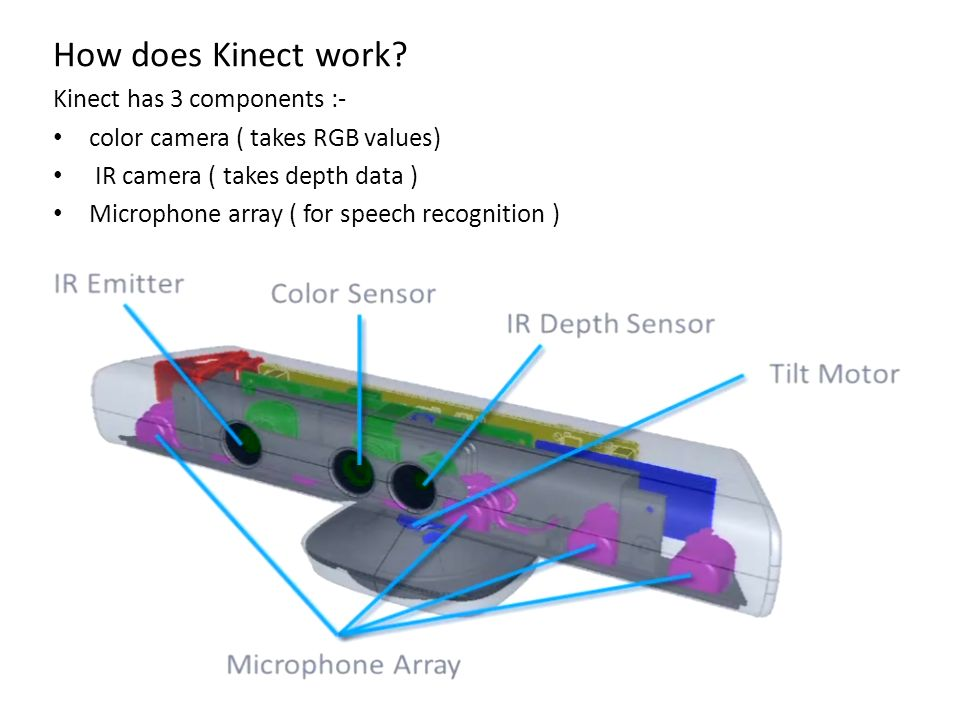
\includegraphics[width=5.5cm, height=3.0cm]{estadoArte/kinect.jpg}	
			\caption{Sensor kinect}
			\end{subfigure}%
			\begin{subfigure}[t]{.5\textwidth}
			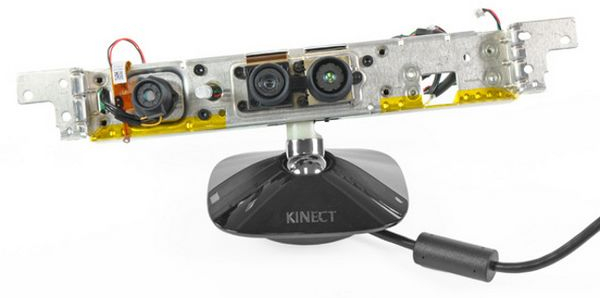
\includegraphics[width=6.5cm, height=3.0cm]{estadoArte/kinect_2.jpg}
			\caption{Sensor kinect estructura}
			\end{subfigure}

			\caption{Sensor kinect elaborado por Microsoft.}

		\end{figure}

		%%\subsection{Características de las imágenes RGB-D}



	\section{Algoritmo RANSAC}
		\subsection{Algoritmo}
		El algoritmo RANSAC (RANdom Sample And Consensus) fue introducido por primera vez por Fischler y Bolles en 1981, como un método para estimar los parámetros de un determinado modelo a partir de un conjunto de datos contaminados por grandes cantidades de outliers. Un dato es considerado un outlier si no encaja en el modelo propuesto, dentro de un umbral de error que define el valor máximo desviación atribuible al efecto del ruido.\\

		RANSAC selecciona uniformemente al azar un subconjunto de muestras de datos y lo utiliza para crear un modelo de estimación de parámetros. Luego determina si las muestras que están dentro de una tolerancia de error del  modelo antes propuesto. Si estas muestras se consideran como parte del modelo generado se agrupan en un conjunto llamado \textit{consenso}. De manera análoga se llama \textit{outliers} al conjunto de tos que superan el umbral de error con respecto al modelo. Si el recuento de los datos agrupados en el consenso es suficientemente alto con respecto de los outliers, se considera que el modelo se ajusta al conjunto de datos, siendo el modelo propuesto un modelo que se aproxima al conjunto total de datos.\\

		A continuación se muestra el seudocódigo básico para el algoritmo RANSAC.\\

		
		\noindent\fbox{
		\begin{minipage}{1.0\textwidth}\scriptsize
		\begin{algorithmic}
			
			\State{Parámetros:}
			    \State{datos – conjunto de datos observados}
			    \State{modelo – una propuesta de modelo que puede ajustar al conjunto de datos}
			    \State{n – el número mínimo de datos con los cuales se considera un buen modelo}
			    \State{k – el número máximo de iteraciones para algoritmo}
			    \State{t – el valor del umbral que determinará si un punto se justa al modelo}\\

			\State{Salidas:}
			    \State{mejorAjuste – modelo encontrado con los parámetros o una variable vacía si no se encontró ningún modelo que justara.}\\

			\State{Inicialización de variables:}
			\State{iteraciones = 0}
			\State{mejorModelo = vacío}
			\State{mejorError = Algo realmente grande}\\
			

		
			\While{ $iteraciones < k$}
				\State{Generación del modelo a partir de datos aleatoriamente seleccionados.}
			    \State{$modeloPropuesto = f(datos)$}
			    \State{inliers = 0}

			    \For{ cada punto \textbf{in} datos \textbf{ and not} en inliers }
			    	\State{calcular error}
			        \If{ punto ajusta en modeloPropuesto \textbf{with an} error $<$ \textbf{than} t}
			            \State{añadir punto a inliers}
			            \State{errorModelo = errorModelo + error }
			        \EndIf{}
			    \EndFor{}\\

			    \If{ número de elementos \textbf{in} inliers $is > n$} 
			        \State{\textit{esto significa que tenemos un buen modelo} }

			        \State{\textit{Verificamos si el modelo calculado supera al mejor modelo calculado con anterioridad.} }
			        \If{ errorModelo $<$ mejorError}
			            \State{mejorAjuste = mejorModelo}
			            \State{mejorError = errorModelo}
			        \EndIf{}
			    \EndIf{}
			    
			    \State{incrementamos iteraciones}
			\EndWhile{}

			\State{\textit{Llegamos al numero de iteraciones k y devolvemos el mejor modelo obtenido.}}\\

			\State{\textbf{return} mejorAjuste}
		\end{algorithmic}
		
		\end{minipage}
		}


		\subsection{Modelo matemático de un plano}
		En matemáticas, un plano es una superficie plana, bidimensional que se extiende infinitamente lejos. Un plano es el análogo bidimensional de un punto (dimensiones cero), una línea (una dimensión) y un espacio tridimensional. Los planos pueden surgir como subespacios de algún espacio de dimensión superior, como si las paredes de una habitación estuviesen extendidas infinitamente, o pudieran disfrutar de una existencia independiente por derecho propio, como en el caso de la geometría euclidiana.\\

		Cuando se trabaja exclusivamente en el espacio euclidiano bidimensional, se utiliza el artículo definido, por lo que el plano se refiere a todo el espacio. Muchas tareas fundamentales en matemáticas, geometría, trigonometría, teoría de gráficas y representación gráfica se realizan en un espacio bidimensional, o, en otras palabras, en el plano.\\

		
		En un espacio euclidiano de cualquier número de dimensiones, un plano está determinado únicamente por cualquiera de los siguientes:\\

		\begin{itemize}
	    	\item{Tres puntos no colineales (puntos no en una sola línea).}
    		\item{Una línea y un punto no en esa línea.}
    		\item{Dos líneas distintas, pero que se cruzan.}
    		\item{Dos líneas paralelas.}
    	\end{itemize}


		Las siguientes afirmaciones se mantienen en el espacio euclidiano tridimensional, pero no en las dimensiones superiores, aunque tienen análogos de mayor dimensión:\\

		\begin{itemize}
			\item{Dos planos distintos son paralelos o se intersecan en una línea.}
	    	\item{Una línea es paralela a un plano, lo cruza en un solo punto, o está contenida en el plano.}
	    	\item{Dos líneas distintas perpendiculares al mismo plano deben ser paralelas entre sí.}
	    	\item{Dos planos distintos perpendiculares a la misma línea deben ser paralelos entre sí.}
	    \end{itemize}

		\section{Forma punto-normal y forma general de la ecuación de un plano}

		De manera análoga a la forma en que se describen las líneas en un espacio bidimensional utilizando una forma de pendiente de puntos para sus ecuaciones, los planos en un espacio tridimensional tienen una descripción natural que utiliza un punto en el plano y un vector ortogonal a él (Vector normal) para indicar su \textit{inclinación}.\\

		Específicamente, sea $r_0$ el vector de posición de algún punto $P_0 = (x_0, y_0, z_0)$, y sea $n = (a, b, c)$ un vector no nulo. El plano determinado por el punto $P_0$ y el vector n consiste en aquellos puntos $P$, con el vector de posición $r$, de tal manera que el vector trazado de $P_0$ a $P$ sea perpendicular a $n$. Recordando que dos vectores son perpendiculares si y sólo si su producto punto es cero, se deduce que el plano deseado puede ser descrito como el conjunto de todos los puntos $r$ tales que:\\

		\begin{equation}
		\begin{split}
		    n.(r-r_0) = 0
	    \end{split}
	    \end{equation}

		(El punto aquí significa un producto punto, no la multiplicación escalar.) Ampliado esto se convierte\\

		\begin{equation}
			\begin{split}
	    	A (x - x_0) + B(y - y_0) + C(z - z_0) = 0
			\end{split}
		\end{equation}

		Que es la forma punto-normal de la ecuación de un plano. Esta es sólo una ecuación lineal\\

		\begin{equation}
			\begin{split}
	    	ax + by + cz + d = 0
	    	\end{split}
    	\end{equation}
		
		donde:\\

		\begin{equation}
			\begin{split}
			d = - (ax_0 + by_0 + cz_0)
	    	\end{split}
    	\end{equation}

		Es un plano que tiene como vector el vector $n = (a, b, c)$. Esta ecuación familiar para un plano se llama la forma general de la ecuación del plano.

		\begin{figure}[h!]
			\begin{center}
			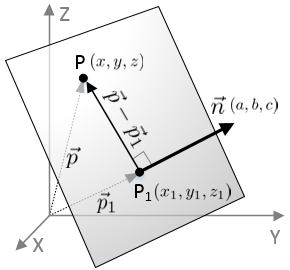
\includegraphics[width=7.5cm, height=6.0cm]{planes/planeEquation.png}	
			\caption{Ecuación de un plano definido por un punto y su normal.}
			\end{center}
		\end{figure}

		\subsection{Modelo del plano definido por tres puntos}

		Sea $p_1=(x_1, y_1, z_1)$, $p_2=(x_2, y_2, z_2)$, y $p_3=(x_3, y_3, z_3)$ puntos en el espacio $R^3$ no-colineales.\\

		Este plano también puede ser descrito por el "punto y un vector normal" de acuerdp  a la descripción anterior. Un vector normal adecuado se da por el producto cruz.\\
		
		\begin{equation}
			\begin{split}
			n = (p_2 - p_1) \times (p_3 - p_1)
			\end{split}
		\end{equation}

		Y el punto $r_0$ puede considerarse como cualquiera de los puntos dados $p_1$, $p_2$ o $p_3$ (o cualquier otro punto en el plano).\\
		

		\textbf{Distancia desde un punto a un plano.}\\

		Para un plano $\Pi: ax + by + cz + d = 0$ y un punto $P_1 = (x_1, y_1, z_1)$ no necesariamente en el plano, la distancia más corta de $P_1$ al plano es\\

		\begin{equation}
			\begin{split}
			D = \dfrac{| ax_1 + by_1 + cz_1 + d |}{\sqrt{a^2 + b^2 + c^2}}
			\end{split}
		\end{equation}

		De lo cual podemos observar que el punto $p_1$ se encuentra en el plano si y sólo si $D = 0$.\\

		Si $\sqrt{a^2 + b^2 + c^2} = 1$ significa que a, b, y c están normalizados,  entonces la ecuación se convierte en:\\
		
		\begin{equation}
			\begin{split}
			D = | ax_1 + by_1 + cz_1 + d |
			\end{split}
		\end{equation}


	\section{Algoritmo PCA}
		El Análisis de Componentes Principales (PCA) ha sido llamado Uno de los resultados más valiosos de la álgebra lineal. PCA Se usa abundantemente en muchas formas de análisis, desde la neurociencia a la computación gráfica debido a que es un método simple. El PCA proporciona una metodología para reducir un conjunto de datos complejos a una dimensión inferior.\\	

		El algoritmo PCA tiene sus bases en las estadísticas y parte de la idea de que se cuenta con un gran conjunto de datos, y desea analizar ese conjunto en términos de las relaciones entre los puntos individuales dentro de ese conjunto de datos. Se pretende analizar algunas de las medidas que podemos calcular en un conjunto de datos, y lo que estás medidas dicen acerca de los datos en sí.\\

		El tema entero de las estadísticas se basa en la idea de que usted tiene este gran conjunto de datos, Y desea analizar ese conjunto en términos de las relaciones entre un puntos de ese conjunto y el resto de los datos. A continuación se intenta explicar las matemáticas detrás de PCA.\\
	
		\subsection{Desviación estándar}
		
			La desviación estándar es una medida de la dispersión de un conjunto de datos respecto de la media. Se calcula como la raíz cuadrada de la varianza, determinando la variación entre cada punto perteneciente al conjunto de  datos respecto a la media. Si los puntos de datos están más lejos de la media, hay una desviación más alta dentro del conjunto de datos.\\

			%%%%%%TEORIA SOBRE DESVIACIONES ESTANDART %%%%%%
			Dado que la desviación estándar puede ser interpretada como una medida de incertidumbre cuando cálculamos el valor de esta en un grupo repetido de medidas nos da la precisión de éstas. Cuando se va a determinar si un grupo de medidas está de acuerdo con el modelo teórico, la desviación estándar de esas medidas es de vital importancia: si la media de las medidas está demasiado alejada de la predicción (con la distancia medida en desviaciones estándar), entonces consideramos que las medidas contradicen la teoría. Esto es coherente, ya que las mediciones caen fuera del rango de valores en el cual sería razonable esperar que ocurrieran si el modelo teórico fuera correcto. La desviación estándar es uno de tres parámetros de ubicación central; muestra la agrupación de los datos alrededor de un valor central (la media o promedio).\\
			%%%%%%%%%%%%%%%%%%%%%%%%%%%%%%%%%%%%%%%%%%%%%%%%%%
			%%%%%%%%%%%%%%%%%%%%%%%%%%%%%%%%%%%%%%%%%%%%%%%%%%

			Por tanto para calcular la desviación estándar primero debemos calcular la media del conjunto de datos.\\

			Cálculo de la media de un conjunto de datos.\\
			
			\begin{equation}
				\begin{split}
					\bar{X} = \dfrac{\Sigma^n_{i=1} X_i}{n}
				\end{split}
			\end{equation}

			Donde $n$ es el numero total de datos contenido en la muestra.\\
			
			Cálculo de la desviación estándar.\\
			\begin{equation}
				\begin{split}
					\sigma = \sqrt{\dfrac{\Sigma^n_{i=1} (X_i - \bar{X})^2} {(n-1)} }
				\end{split}
			\end{equation}


			\begin{figure}
				\begin{center}
				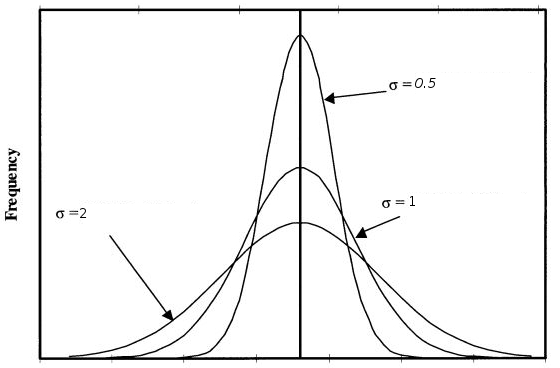
\includegraphics[width=10.5cm, height=7.0cm]{estadoArte/standarDeviation4.jpg}	
				\caption{Distribución normal con media cero y diferentes desviaciones estándar.}
				\end{center}
			\end{figure}



		\subsection{Varianza}
			La noción de varianza se suele emplear en el ámbito de la estadística. Es utilizada para identificar a la media de las desviaciones cuadráticas de una variable de carácter aleatorio, considerando el valor medio de ésta.\\

			
			La varianza de las variables aleatorias, por lo tanto, consiste en una medida vinculada a su dispersión. Se trata del valor esperado del cuadrado de la desviación de esa variable considerada frente su media y se mide en una unidad diferente. Por ejemplo: en los casos en que la variable mide una distancia en kilómetros, su varianza se expresa en kilómetros al cuadrado.\\

			Cabe destacar que las medidas de dispersión (también identificadas con el nombre de medidas de variabilidad) se encargan de expresar la variabilidad de una distribución por medio de un número, en los casos en que las diferentes puntuaciones de la variable están muy alejadas de la media. A mayor valor de la medida de dispersión, mayor variabilidad. En cambio, a menor valor, más homogeneidad.\\

			Por lo que respecta a su representación matemática se puede expresar como el cuadrado del valor de la desviación estándar, como se muestra a continuación.\\ 

			\begin{equation}
				\begin{split}
					s = \sigma^2
				\end{split}
			\end{equation}

			\begin{equation}
				\begin{split}
					s = \dfrac{\Sigma^n_{i=1} (X_i - \bar{X})^2} {(n-1)}
				\end{split}
			\end{equation}

		\subsection{Covarianza}
		
			Las dos últimas medidas que hemos observado son puramente uni-dimensionales. Conjuntos de datos como este podrían ser: alturas de todas las personas en la sala, las calificaciones para el último examen, etc. Sin embargo, muchos conjuntos de datos tienen más de una dimensión y el objetivo del Análisis de Componentes Principales son estos conjuntos de datos. En tal caso es importante observar si existe alguna relación entre las diferentes dimensiones. Por ejemplo, podríamos tener como nuestro conjunto de datos tanto la altura de todos los estudiantes en una clase, y la calificación  que recibieron en un examen.\\ 

			Podríamos entonces realizar un análisis estadístico para ver si la altura de un estudiante tiene algún efecto en su calificación. La desviación estándar y la varianza sólo funcionan en una dimensión, de modo que podríamos solamente calcular la desviación estándar para cada dimensión del conjunto de datos de forma independiente de las otras dimensiones. Sin embargo, es útil tener una medida similar para mucho las dimensiones varían de la media con respecto a la otra. La covarianza es tal medida. Covarianza siempre se mide entre 2 dimensiones. Si se calcula la covarianza entre una dimensión y sí, se obtiene la diferencia.\\


			Por lo tanto, si se tiene un conjunto de datos en 3 dimensiones $(x, y, z)$, entonces se podría medir la covarianza entre: las dimensiones $(x, y)$, las dimensiones $(x, z)$ y las dimensiones $(y, z)$. Como se puede observar la medición de la covarianza entre $(x, x)$, $(y, y)$ o $(z, z)$ se puede reducir a calcular la varianza de cada dimensión respectivamente. La fórmula para la covarianza es muy similar a la fórmula para la varianza. La formula:\\ 

			\begin{equation}
				\begin{split}
					var(X) = \dfrac{\Sigma^n_{i=1} (X_i - \bar{X} ) (X_i - \bar{X}) } {(n - 1)}
				\end{split}
			\end{equation}

			\begin{equation}
			\begin{split}
				cov(X, Y) = \dfrac{\Sigma^n_{i=1} (X_i - \bar{X} ) (Y_i - \bar{Y}) } {(n - 1)}
			\end{split}
			\end{equation}


		\subsection{Matriz de covarianzas}
		
			Cuando se dispone de un conjunto de datos multidimensionales la información obtenida de los cálculos de las covarianzas se dispone en forma de matriz para facilitar su manejo, tal matriz es llamada \textit{Matriz de covarianzas}. La matriz de covarianzas es de dimensiones $n \times n$ donde n es el número de dimensiones totales en el conjunto de datos.\\

			A continuación se muestra la matriz de covarianzas para un conjunto de datos de 3 dimensiones, llamadas $x, y,$ y $z.$


			\begin{equation}
				C =
				\begin{bmatrix}
	    			cov(x, x) & cov(x, y) & cov(x, z) \\
				    cov(y, x) & cov(y, y) & cov(y, z) \\
				    cov(z, x) & cov(z, y) & cov(z, z)
				\end{bmatrix}
			\end{equation}

		\subsection{Eigenvalores y Eigenvectores}

			Se conocen como valores propios de una matriz al conjunto de valores que resuelven la ecuación:\\

			\begin{equation}
				\begin{split}
					|A - \lambda I | = 0
				\end{split}
			\end{equation}

			\begin{equation}
				\begin{split}
					det( A - \lambda I ) = 0
				\end{split}
			\end{equation}

			También puede observarse que $\lambda$ es un vector de valores escalares que a su vez son solución del polinomio de grado $n$. Donde $n$ es la dimensión de la matriz $A$: \\

			Polinomio característico.\\
			\begin{equation}
				| A - \lambda I | = (\lambda_1 - \lambda) (\lambda_2 - \lambda) (\lambda_3 - \lambda)... (\lambda_n - \lambda)
			\end{equation}

			
			Por lo tanto, existe un eigenvector asociado a cada uno de los valores propios de la matriz A\\
			
			\begin{equation}
				\begin{split}
					( A - \lambda I )v = 0
				\end{split}
			\end{equation}


			Para encontrar el valor de los vectores característicos de la matriz A se determinan los valores característicos de la matriz A se resuelve la ecuación:\\

			
			\begin{equation}
				\begin{split}
					(A - \lambda_1 I) \vec{v_1} = 0 \\
					(A - \lambda_2 I) \vec{v_2} = 0 \\
					. \\
					. \\
					. \\
					(A - \lambda_3 I) \vec{v_n} = 0 
				\end{split}
			\end{equation}

			Es importante observar que el conjunto de todos los vectores propios asociados a un valor propio dado $\vec{E_\lambda}$, junto con el vector 0 , forman un espacio vectorial.\\

			Por lo tanto, $\vec{E_\lambda}$ representa un subespacio de $R^n$ porque es el espacio solución de un sistema homogéneo de ecuaciones lineales y está conformado por  matrices columna $\vec{v}$ de $n x 1$ que pertenecen a $R^n$.\\

			Los vectores característicos $\vec{v_1}, \vec{v_2}, \vec{v_2} ... \vec{v_n}$ , asociados a los valores característicos distintos $\lambda_1, \lambda_2, ...\lambda_n$ de la matriz A, \textbf{son linealmente independientes, y este conjunto es una base en $R^n$}. Si la matriz A es simétrica y real, entonces las base es ortogonal.\\

			Es importante resaltar estas dos características puesto que la aplicación que se desarrollará en este trabajo se basa en el principio de la independencia lineal de los vectores propios y que estos construyen una base ortogonal del conjunto de datos observados.



%%%%%%%%%%%%%%%%%%%%%%%%%%%%%%%%%%%%%%%%%%%%%%%%%%
%%%%%	\section{Características del objeto}



%%%%%%%%%%%%%%%%%%%%%%%%%%%%%%%%%%%%%%%%%%%%%%%%%%
%%%%	\section{Planeación de tareas}

